\documentclass{article}
\usepackage{graphicx}
\usepackage{subfigure}
\usepackage{amsmath}
\usepackage[letterpaper]{geometry}
\title{Smoothing polylines with circles}
\author{Jason Sewall}
\date{October 4, 2009}
\begin{document}
\maketitle

\section{Smoothing two-dimensional polylines}

\subsection{The problem}
We have an ordered sequence $P$ of $n$ 2D points:

\begin{equation}
  \label{eq:points}
  P := \left(p_{0}, p_{1},\ldots,p_{n-2},p_{n-1}\right)
\end{equation}

These points define a (planar) polyline with $n-1$ segments such as that in Fig.~\ref{fig:polyline}.  Let us assume that there are no two points adjacent in the sequence that are equal, and that there are no three adjacent points that are colinear; clearly we can eliminate these adjacent repeated points or the central points in a colinear sequence without modifying the line's shape.

\begin{figure}[h]
  \centering
  \subfigure[\label{fig:polyline} A polyline $P$]{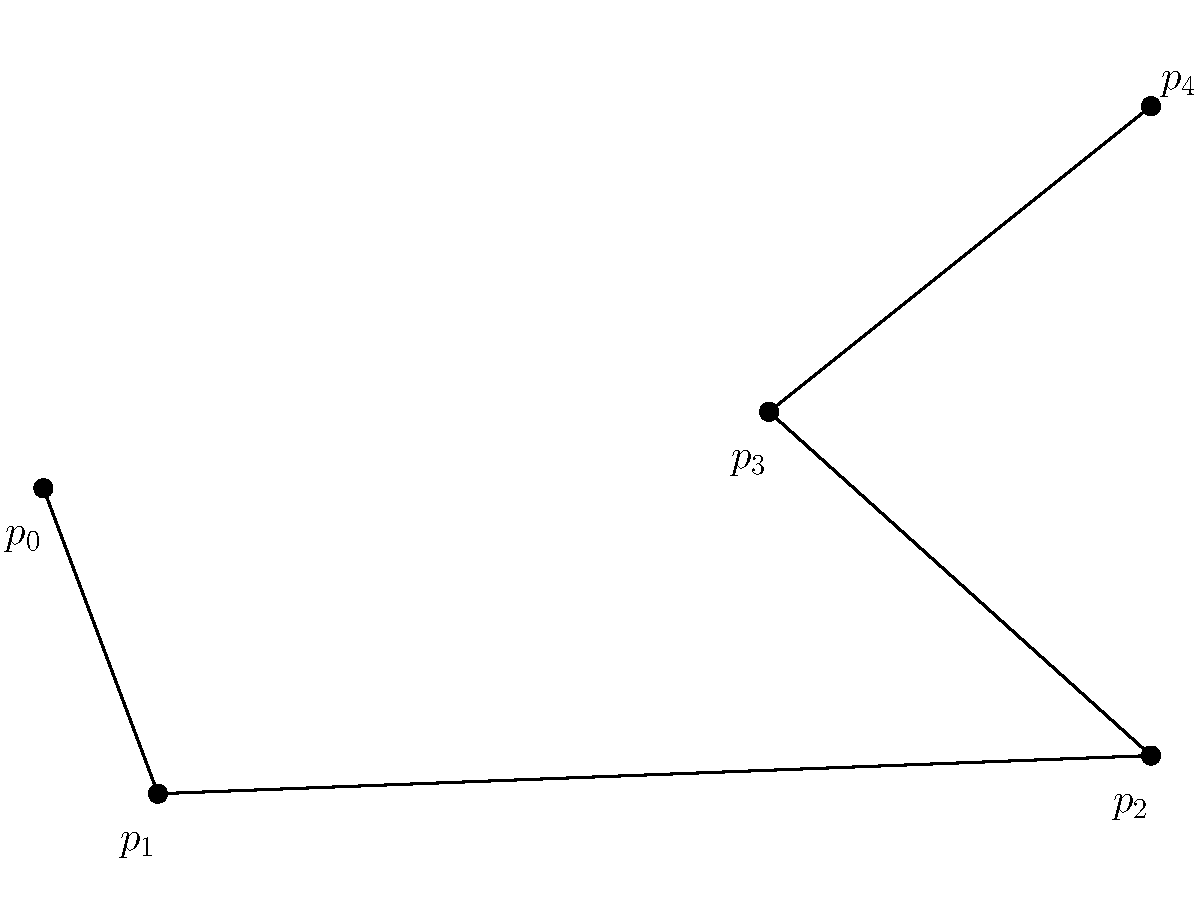
\includegraphics[width=7cm]{1}}\hfill
  \subfigure[\label{fig:smooth-polyline}$P_S$: A `smoothed' version of the polyline $P$]{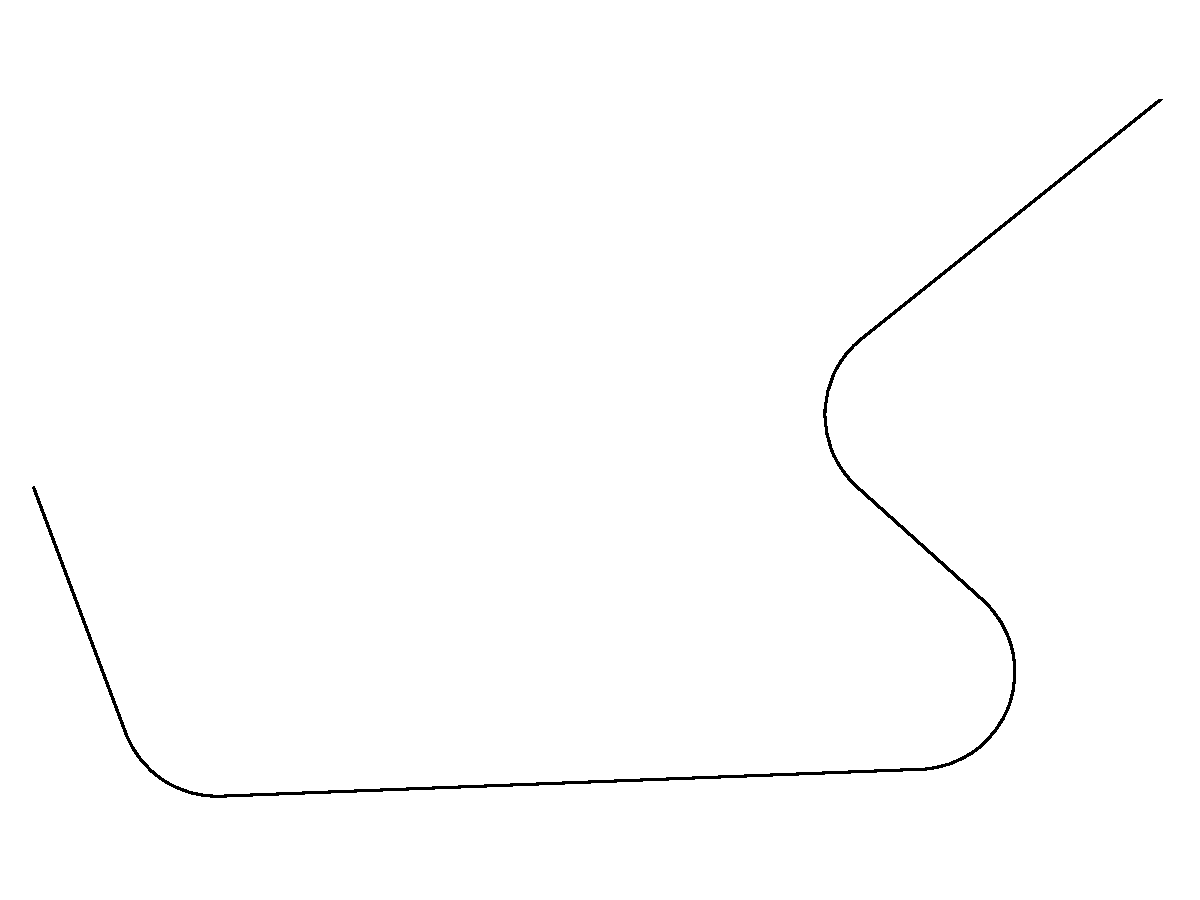
\includegraphics[width=7cm]{2}}\\
  \subfigure[\label{fig:debug-smooth-polyline}The polyline $P$ and the circles defining $P_S$]{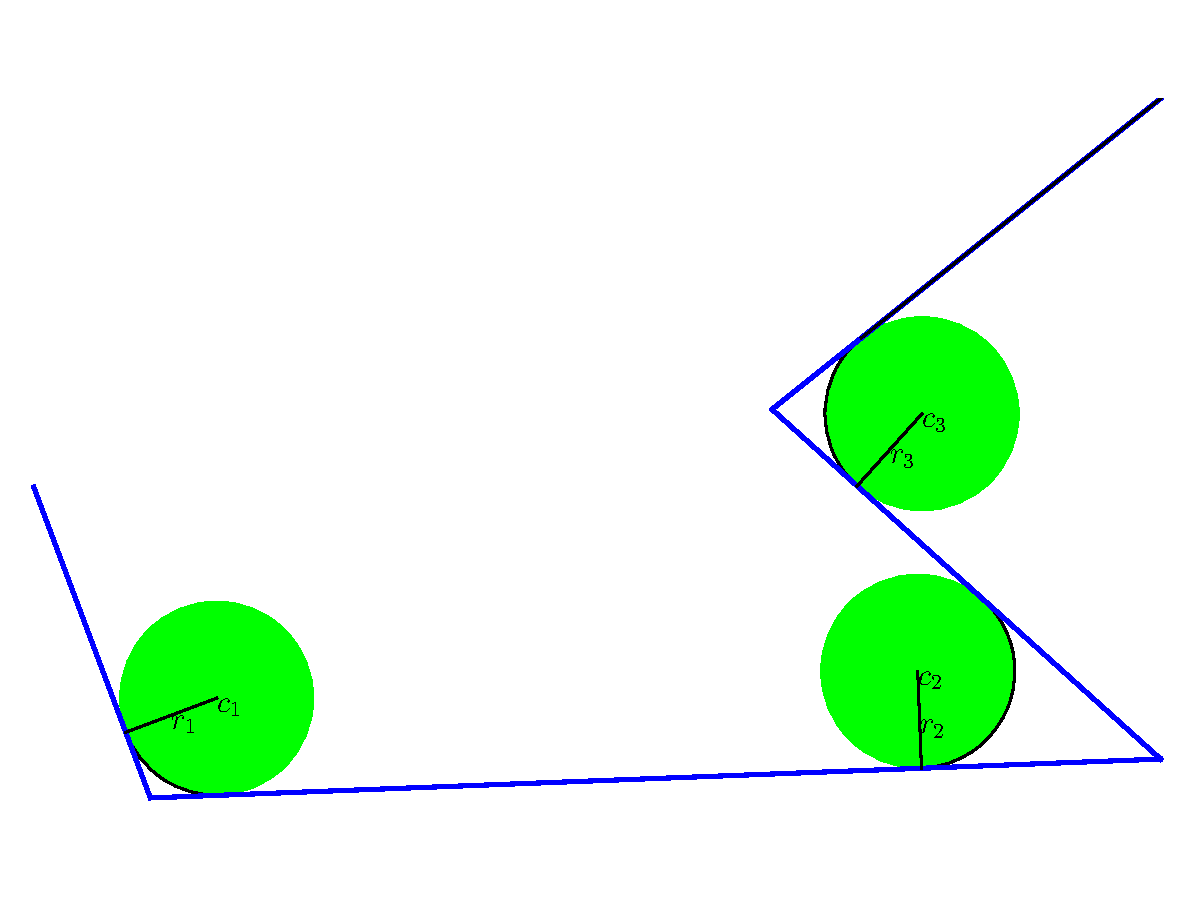
\includegraphics[width=7cm]{3}}
  \caption{Polylines}
\end{figure}

We wish to `smooth' this polyline to something like what is shown in Fig.~\ref{fig:smooth-polyline}, which we shall refer to as $P_S$.  We construct $P_S$ by replacing the region around each interior point $p_{i}, i \in \mathbb{Z}\left[1, n-2\right]}$ of $P$ with a circular arc $\mathbf{a}_{i}$ and retaining the exterior points $p_0$ and $p_{n-1}$.  We abuse notation slightly and define

\begin{equation}
  \label{eq:p-smooth}
  P_S := \left(p_0, a_1, a_2, a_{n_2}, \ldots, p_{n-1}\right)
\end{equation}

Where each $\mathbf{a}_{i}$ is defined by:

\begin{equation}
  \label{eq:circ-def}
\mathbf{a}_i=\left(
  c_{i},
  r_{i},
  \theta^{0}_{i},
  \theta^{1}_{i}
\right)
\end{equation}

And here $c_{i}$ is the center, $r_{i}$ is the radius, and $\theta^{0}_{i}, \theta^{1}_{i}$ are the angular extents of the arc.  See Fig. \ref{fig:debug-smooth-polyline}; each $\mathbf{a}_{i}$ is shown.



\subsection{Formulation of the arcs $a_{i}$}

\subsubsection{Definitions}

For each interior point $p_{i}$, the associated arc $\mathbf{a}_{i}$ is determined closely associated with the triple of points:

\begin{equation}
  \label{eq:arc-triple}
  T_{i} = \left(p_{i-1}, p_{i}, p_{i+1}\right)
\end{equation}

\paragraph{Vectors}

In particular, we are interested in the derived vectors

\begin{align}
  \label{eq:vector-b}
  \mathbf{v}^{b}_{i} &= p_{i-1} - p_{i}\\
  \label{eq:vector-f}
  \mathbf{v}^{f}_{i} &= p_{i+1} - p_{i}
\end{align}

their lengths:

\begin{align}
  \label{eq:vector-length-b}
  L^{b}_{i} &= \left|\mathbf{v}^{b}_{i}\right|\\
  \label{eq:vector-length-f}
  L^{f}_{i} &= \left|\mathbf{v}^{f}_{i}\right|
\end{align}

and the associated unit vectors:

\begin{align}
  \label{eq:unit-vector-b}
  \mathbf{n}^{b}_{i} &= \frac{\mathbf{v}^{b}_{i}}{L^{b}_{i}} &=\frac{\mathbf{v}^{b}_{i}}{\left|\mathbf{v}^{b}_{i}\right|}\\
  \label{eq:unit-vectors-f}
  \mathbf{n}^{f}_{i} &= \frac{\mathbf{v}^{f}_{i}}{L^{f}_{i}} &=\frac{\mathbf{v}^{f}_{i}}{\left|\mathbf{v}^{f}_{i}\right|}
\end{align}

\paragraph{Tangent points}

The projections of $c_{i}-p_{i}$ onto $\mathbf{n}^{b}_{i}$ and onto $\mathbf{n}^{f}_{i}$ have equal length $\alpha_i$; then the tangent points of the circle on $\mathbf{v}^{b}_{i}$ and $\mathbf{v}^{b}_{i}$ are:

\begin{align}
  \label{eq:alpha-vector-b}
  \left(c_{i}-p_{i}\right)\;\mathrm{proj}\; \mathbf{n}^{b}_{i} &= \alpha_i\mathbf{n}^{b}_{i}\\
  \label{eq:alpha-vector-f}
  \left(c_{i}-p_{i}\right)\;\mathrm{proj}\; \mathbf{n}^{f}_{i} &= \alpha_i\mathbf{n}^{f}_{i}
\end{align}

\paragraph{Radius vectors}

We are also interested in the (negative) radius vectors from these points to the center $c_{i}$:

\begin{align}
  \label{eq:radius-vector-b}
  \mathbf{r}^{b}_{i} &= c_{i} - \left(\alpha\mathbf{n}^{b}_{i} - p_{i}\right)&=\pm r_i\left( -{\mathbf{n}^{b}_{i}}_{y},  {\mathbf{n}^{b}_{i}}_{x} \right)\\
  \label{eq:radius-vector-f}
  \mathbf{r}^{f}_{i} &= c_{i} - \left(\alpha\mathbf{n}^{f}_{i} - p_{i}\right)&=\pm r_i\left(  {\mathbf{n}^{f}_{i}}_{y}, -{\mathbf{n}^{f}_{i}}_{x} \right)
\end{align}

Obviously, $\left|\mathbf{r}^{b}_{i}\right| = \left|\mathbf{r}^{f}_{i}\right| = r_{i}$.

The sign of the rightmost term in Eqs.~\eqref{eq:radius-vector-b},~\eqref{eq:radius-vector-f} ($\pm$) is determined by the orientation of the triple $T_i$ (see Eqs.~\eqref{eq:vector-b}, ~\eqref{eq:vector-f}); that is to say:

\begin{equation}
  \label{eq:orientation}
  o_i = \mathrm{sign}\; \mathbf{n}^{b}_{i} \times \mathbf{n}^{f}_{i}
\end{equation}

\paragraph{The center}

The center $c_{i}$ can be determined by combining Eqs.~\eqref{eq:radius-vector-b},~\eqref{eq:radius-vector-f} and~\eqref{eq:alpha-vector-b}, ~\eqref{eq:alpha-vector-f}:

\begin{align}
  \label{eq:center-vector-b}
  c_{i} &= p_{i} + \alpha_i\mathbf{n}^b_i + \mathbf{r}^{b}_{i}\\
  \label{eq:center-vector-f}
  c_{i} &= p_{i} + \alpha_i\mathbf{n}^f_i + \mathbf{r}^{f}_{i}
\end{align}

We can also write $c_{i}$ in terms of the unit bisector $\mathbf{b}_{i}$:

\begin{equation}
  \label{eq:center-bisector}
  c_{i} = p_{i} + \sqrt{r_{i}^{2} + \alpha_{i}^{2}}\mathbf{b}_{i}
\end{equation}

Where $\mathbf{b}_i$ is of course given by:

\begin{equation}
  \label{eq:bisector}
  \mathbf{b}_i = \frac{\mathbf{n}^b_i + \mathbf{n}^f_i}{\left|\mathbf{n}^b_i + \mathbf{n}^f_i\right|}
\end{equation}

See Fig.~\ref{fig:interior-point} for a visual depiction of these quantities.

\begin{figure}[h]
  \centering
  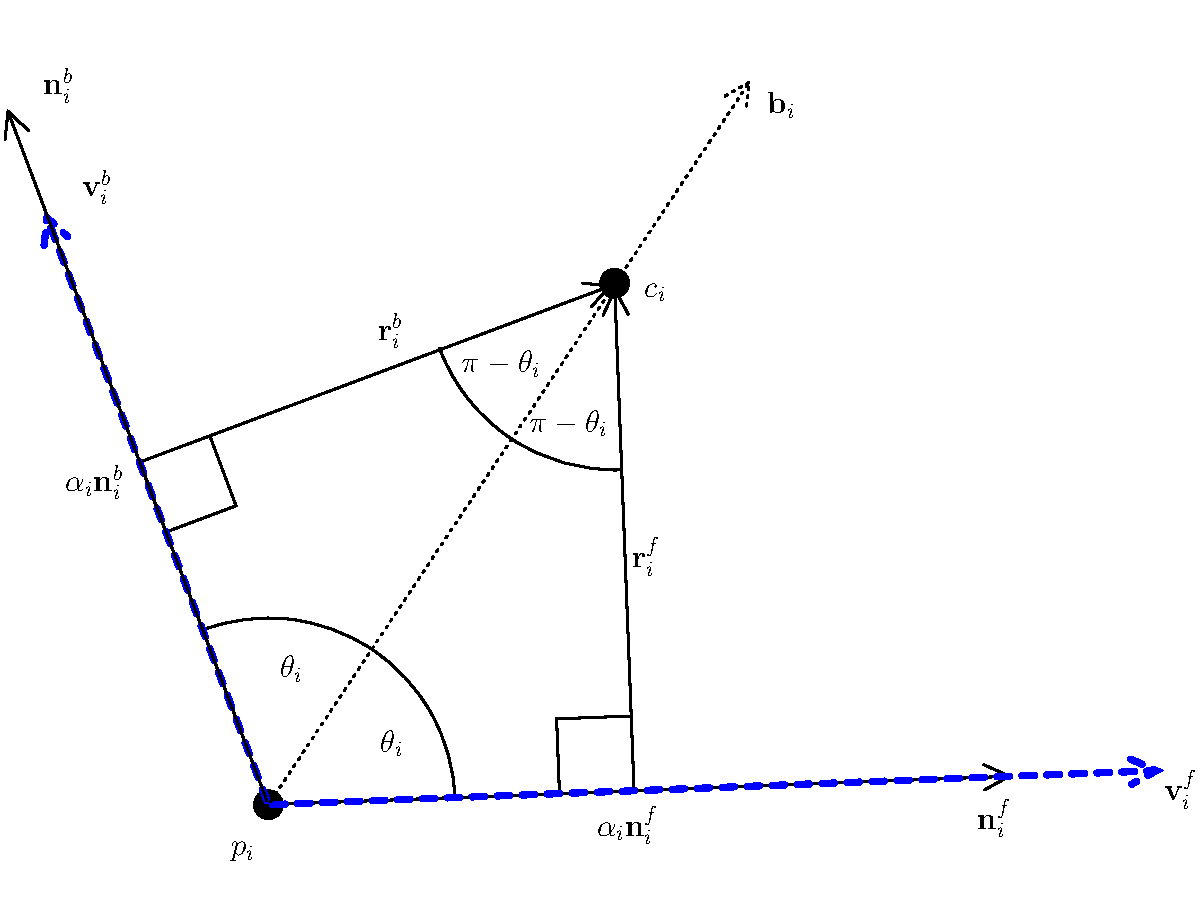
\includegraphics[width=\columnwidth]{4}
  \caption{The interior point $p_{i}$ with backward vector $\mathbf{v}^{b}_{i}$ and forward vector $\mathbf{v}^{f}_{i}$. $\mathbf{b}_{i}$ is the unit bisector of these vectors}
  \label{fig:interior-point}
\end{figure}

\subsubsection{Angles}

For a given $T_i$, the arc angles $\theta^0_i$ and $\theta^{1}_{i}$; are fixed regardless of the $c_i$ or $r_{i}$:

\begin{align}
  \label{eq:angle-range-b}
  \theta^{0}_{i} &= \arctan \frac{{\mathbf{r}^{b}_{i}}_{y}}{{\mathbf{r}^{b}_{i}}_{x}}\\
  \label{eq:angle-range-f}
  \theta^{1}_{i} &= \arctan \frac{{\mathbf{r}^{f}_{i}}_{y}}{{\mathbf{r}^{f}_{i}}_{x}}
\end{align}

The total arc length of $a_i$ (the angle $\left|\theta^0_i -\theta^1_i\right|$) is given by $2\left(\pi-\theta_i\right)$ (see Fig.~\ref{fig:interior-point})

We can also relate the input vectors for a given $T_{i}$ to $\theta$:

\begin{equation}
  \label{eq:dotnorm}
  \mathbf{n}^{f}_{i} \cdot \mathbf{n}^{b}_{i} = \cos 2\theta_i
\end{equation}

Similarly, we know

\begin{align}
  \notag
  \left|\theta^0_i -\theta^1_i\right| &= 2\left(\pi-\theta_i\right)\\
  \label{eq:arclen-dot}
  &= 2\pi-\arccos \mathbf{n}^{f}_{i} \cdot \mathbf{n}^{b}_{i}
\end{align}

Clearly, Eqs.~\eqref{eq:angle-range-b},~\eqref{eq:angle-range-f} and~\eqref{eq:dotnorm} are independent of other arc parameters $c_{i}$, $r_{i}$, and $\alpha_i$.

\subsubsection{Equation for $r_i$ and $\alpha_{i}$}

For a given triple $T_{i}$, we would like a formula relating $r_{i}$, and $\alpha_{i}$.  From visual inspection of Fig.~\ref{fig:interior-point}, we can see that:

\begin{align}
  \notag
  \frac{r_i}{\alpha_{i}} &= \tan \theta_i\\
  \label{eq:tantheta}
  r_i &= \alpha_{i}\tan \theta_i
\end{align}

We know from trigonometry that

\begin{align}
  \notag
  \tan \frac{\phi}{2} &= \sqrt{\frac{1-\cos\phi}{1+\cos\phi}}\\
  \label{eq:tanident}
  \tan \theta &= \sqrt{\frac{1-\cos 2\theta}{1+\cos 2\theta}}
\end{align}

We can combine Eq.~\eqref{eq:tantheta} with Eq.~\eqref{eq:tanident} to obtain

\begin{align}
  \label{eq:radiustan}
  r_{i} &= \alpha_i\sqrt{\frac{1-\cos 2\theta}{1+\cos 2\theta}}
\end{align}

Finally, we can substitute Eq.~\eqref{eq:dotnorm} into Eq.~\eqref{eq:radiustan}, and obtain

\begin{align}
  \label{eq:radius-alpha}
  r_{i} &= \alpha_i\sqrt{\frac{1-\mathbf{n}^f_i\cdot \mathbf{n}^b_i}{1+\mathbf{n}^f_i\cdot \mathbf{n}^b_i}}
\end{align}

\subsection{Length of a smoothed polyline}

It is useful to consider the length of a smoothed polyline $P_S$.  This will be the sum of the circumference of each arc $a_i$ plus the length of the straight line segments connected consecutive arcs and the segments connecting $p_0$ to $a_1$ and $a_{n-2}$ to $p_{n-2}$.

The length $w_i$ of an arc $a_i = \left(c_i, r_i, \theta^0_i, \theta^1_i\right)$ is given by the standard formula:

\begin{equation}
  \label{eq:circumference}
  w_i  = 2\pi r_i \frac{\left|\theta^0_i - \theta^1_i\right|}{2\pi} = r_i \left|\theta^0_i - \theta^1_i\right|
\end{equation}

The length $s_i$ of a segment connecting two consecutive arcs $a_{i-1}$ and $a_i$ is simply the length of the original line from $p_{i-1}$ to $p_i$ minus the $\alpha_{i-1}$ and $\alpha_i$ of $a_{i-1}$ and $a_i$:

\begin{equation}
  \label{eq:seglen}
  s_i = \left|p_i - p_{i-1}\right| - (\alpha_i - \alpha_{i-1})
\end{equation}

If we define $\alpha_0 = \alpha_{n-1} = 0$ for the endpoints $p_0$ and $p_{i-1}$, we can use Eq.~\eqref{eq:seglen} for the beginning/end segments as well.

For nondegenerate $P_S$ (i.e. with $n>2$), we have:

\begin{align}
  \notag
  L\left(P_S\right) &= \sum^{n-2}_{i = 1} r_i\left|\theta^0_i - \theta^1_i\right| + \sum^{n-1}_{i=1} \left|p_i - p_{i-1}\right| - (\alpha_i - \alpha_{i-1})\\
  \label{eq:smoothpoly-len}
  &= L\left(P\right) + \sum^{n-2}_{i = 1} r_i\left|\theta^0_i - \theta^1_i\right| - 2\sum^{n-2}_{i=1} \alpha_i
  % \notag
  % &= L\left(P\right) + \sum^{n-2}_{i = 1} \alpha_i\sqrt{\frac{1-\mathbf{n}^f_i\cdot \mathbf{n}^b_i}{1+\mathbf{n}^f_i\cdot \mathbf{n}^b_i}}\left|\theta^0_i - \theta^1_i\right| - 2\alpha_i\\
  % \label{eq:smoothpoly-len}
  % &= L\left(P\right) + \sum^{n-2}_{i = 1} \alpha_i\left(\sqrt{\frac{1-\mathbf{n}^f_i\cdot \mathbf{n}^b_i}{1+\mathbf{n}^f_i\cdot \mathbf{n}^b_i}}\left|\theta^0_i - \theta^1_i\right| - 2\right)
\end{align}

\subsection{Offset polylines}

So far, given a planar polyline $P$ and either an $\alpha_i$ or $r_i$ for each interior point $P_i$, we can compute the smoothed polyline $P_S = p_0, a_1, a_2,\ldots\,a_{n-2}, p_{n-1}$ by computing the associated circle $a_i=\left(c_i, r_i, \theta^0_i, \theta^1_i\right)$ for each interior point of $P$ using Eq.~\eqref{eq:radius-alpha} to find $r_i$ or $\alpha_i$, one of Eqs.~\eqref{eq:center-vector-b},~\eqref{eq:center-vector-f}, or~\eqref{eq:center-bisector} to find $c_i$, and Eqs.~\eqref{eq:angle-range-b}, and ~\eqref{eq:angle-range-f} for $\theta^0_i$ and $\theta^1_i$.  We retain the original polyline $P$ external points $p_0$ and $p_{n-1}$ as the endpoints of $P_S$.

Suppose we wish to compute a new smoothed polyline $P_S'$ that has the property that at every point, the nearest point on $P_S$ is exactly distance $d$ away and furthermore.  That is, $P_S'$ is `offset' from $P_S$ to one side by a signed distance $d$; see Fig.~\ref{fig:fattened-polyline}.  We used the convention that $d>0$ refers to a `right' offset (the lower blue line in Fig.~\ref{fig:fattened-polyline}) and $d<0$ to a `left' offset (the upper blue line in the same figure).

\begin{figure}[h]
  \centering
  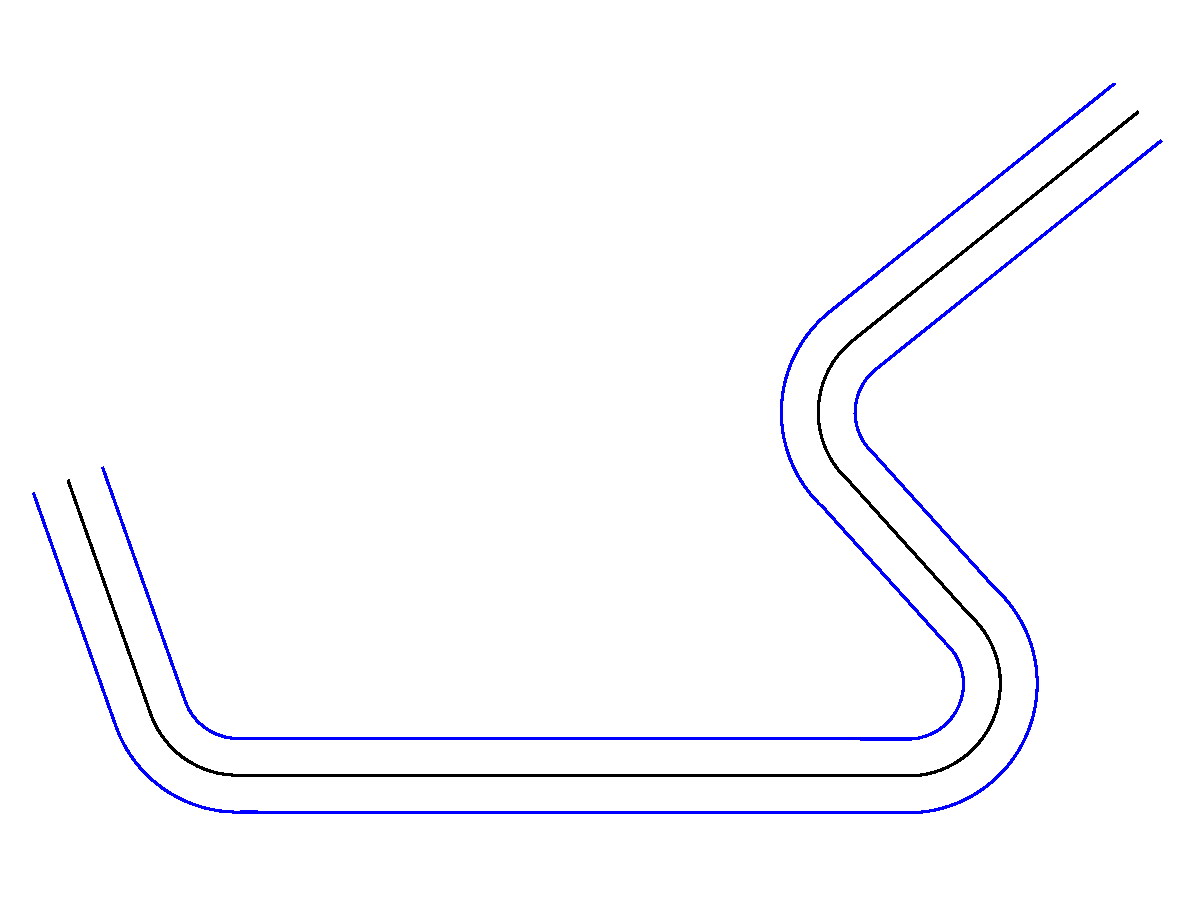
\includegraphics[width=7cm]{5}
  \caption{A `fattened' smoothed polyline; the original smoothed polyline $P_S$ as computed above is drawn in black.  The blue lines represent the same shape offset to either side by an equal distance.}
  \label{fig:fattened-polyline}
\end{figure}

The $a'_i$ corresponding to $P_S'$ (with signed offset $d$) can be derived from $P_S$ by adjusting the $r_i$ by $o_id$, where $o_i$ is given by Eq.~\eqref{eq:orientation}.  That is:

\begin{equation}
  \label{eq:arc-offset}
  a'_i = \left(c_i, r_i + o_id, \theta^0_i, \theta^1_i\right)
\end{equation}

We must also choose new endpoints $p'_0$ and $p'_{n-1}$ for this line;  are the perpendiculars to $n^f_0$ and $n^f_{n-2}$ (from Eq.~\eqref{eq:unit-vectors-f}), scaled and added to $p_0$ and $p_{n-1}$, respectively:

\begin{align}
  \label{eq:endpoints-prime}
  p'_0 &= p_0 + d \left({\mathbf{n}^f_0}_y, -{\mathbf{n}^f_0}_x\right)\\
  p'_{n-1} &= p_{n-1} + d \left(-{\mathbf{n}^f_{n-2}}_y, {\mathbf{n}^f_{n-2}}_x\right)
\end{align}

\subsection{Generating new polyline approximations}


\subsection{Automatic computation of the $r_i$}

\subsubsection{Allowable radii}

For a given $T_{i}$, the range of suitable radii $r_{i}$ depends on $L^b_i$ and $L^f_i$; we can see in Fig.~\ref{fig:interior-point} that were $r_{i}$ to exceed some quantity, one or both of the points of tangency of the circle on the vectors may lie beyond the length(s) of the vectors --- precisely, we require:

\begin{align}
  \label{eq:alphalimit-b}
  \alpha_i &\le L^{b}_{i}\\
  \label{eq:alphalimit-f}
  \alpha_i &\le L^{f}_{i}
\end{align}

\paragraph{Lower bound}

Obviously, $r_i > 0$ to satisfy the usual meaning of a radius.

\paragraph{Upper bound}

To derive an upper bound on $r_{i}$ based on the lengths $L^b_i$ and $L^f_i$, we see in Eq.~\eqref{eq:radius-alpha} that $r_{i}$ is linear in $a_{i}$; thus we need only pick the largest $\alpha_i$ that satisfies Eqs.~\eqref{eq:alphalimit-b} and~\eqref{eq:alphalimit-f}.  This is simply

\begin{equation}
  \label{eq:alpha-max}
  \alpha^{\max}_i = \min \left\{L^{b}_{i}, L^{f}_{i}\right\}
\end{equation}

So for bounds on $r_{i}$, we have

\begin{equation}
  \label{eq:rbounds}
  r_{i} \in \left(0, \alpha^{\max}_i \frac{\sqrt{1-\left(\mathbf{n}^f_i\cdot \mathbf{n}^b_i\right)^{2}}}{1+\mathbf{n}^f_i\cdot \mathbf{n}^b_i}\right]
\end{equation}

\end{document}

%%% Local Variables:
%%% mode: latex
%%% TeX-master: t
%%% End:
